\documentclass[a4paper, 12pt]{article}
\usepackage[utf8]{inputenc}
\usepackage[english,russian]{babel}


\title{Разработка ПО для онлайн монитора светимости детектора Belle II}
\author{Каня Кирилл\\Новосибирский Государствнный Университет}


\begin{document}
\maketitle
\newpage

\tableofcontents
\newpage

\section*{Введение}
Здесь будет введение

\section{Эксперимент Belle II}
    \subsection{Электромагнитный калориметр}
    Здесь будет про электромагнитный калориметр

    \subsection{Онлайн монитор светимости}
    Здусь будет про онлайн монитор светимости

    \subsection{Цель работы}
      При проведении эксперимента Belle II важно контролировать светимость ускорителя, для этой цели в ИЯФ СО РАН был разработан модуль онлайн монитор светимости. Данный модуль измеряет скорость счета $e^+e^-$ рассеяния с торцевых частей электромагнитного калориметра. Измерение светимости в режиме реального времени позволяет получать обратную связь с ускорителем для настройки оптимальных параметров самого ускорителя. Также измерение интеграла светимости позволяет мониторировать процесс набора данных, что является важной задачей при изучении редких распадов, таких как распады $B-$ и $D-$мезонов.
  Данные с монитора светимости представляют интерес для нескольких групп, участвующих в эксперименте Belle II. Каждой группе необходимы различные данные и различная степень детализации этих данных. Следовательно, необходимо ПО, которое позволит каждой группе иметь доступ к этим данным. Таким образом, группы и сценарии использования каждой группой, можно описать следующим образом:
\begin{itemize}

  \item Группа операторов ускорителя. Для получения обратной связи с ускорителя с целью подбора оптимальных значений данной группе требуются следующие значения:
    \begin{itemize}
      \item Мгновенная ускорительная светимость
      \item Интегральные ускорительные светимости за различные промежутки времени
    \end{itemize}

  \item Группа операторов детектора. Для анализа эффективности работы детектора данной группе необходимы следующие значения:
    \begin{itemize}
      \item Получать мгновенную детекторную и ускорительную светимости
      \item Получать аналогичные интегральные светимости за различные промежутки времени 
    \end{itemize}

  \item Группа экспертов по ECL. Для отслеживания корректности работы электромагнитного калориметра данной группе необходимо получать следующие данные:
    \begin{itemize}
      \item Значения пьедесталов для каждого сектора
      \item Формы сигналов с каждого сектора 
      \item Амплитудные гистограммы для каждого сектора 
    \end{itemize}

  \item Группа экспертов по обработке данных. Для отбора заходов по светимостям данной группе необходимы следующие значения:
    \begin{itemize}
      \item Интегральные светимости по заходам
    \end{itemize}

  \item Группа руководителей эксперимента. Данной группе для отслеживания достижения проектных значений светимостей необходимо получать следующие данные:
    \begin{itemize}
      \item Значения интегральных светимостей
      \item Значения максимальных светимостей
    \end{itemize}

\end{itemize}


\section{Программное обеспечение для онлайн монитора светимости}
    \subsection{Интегральные и максимальные значения светимостей}
    Здусь будет про светимости

    \subsection{Расчет пьедесталов}
      Так как монитор светимости работает на базе электромагнитного калориметра, то полученные данные можно использовать для получения обратной связи с электромагнитным калориметром в режиме реального времени. Возможность получения обратной связи полезна тем, что можно оперативно обнаружить неисправности в работе электромагнитного калориметра и устранить их. В частности, для мониторирования уровня шумов электроники удобно использовать значения пьедесталов для каждого сектора. В общем случае пьедестал это отклонение уровня сигнала от нулевого положения.\par
  Для каждого из 32 секторов монитор светимости получает аналоговую сумму сигналов с 2 триггерных ячеек. Соответственно, имея форму сигнала, можно определять отклонение от нулевого положения для каждого сектора в режиме реального времени. Форма сигнала представляет собой массив из 2048 значений на один сектор. Расчет происходит следующим образом:
\begin{enumerate}
  \item Считываем формы сигналов с монитора светимости
  \item Находим максимальное значение в массиве
  \item Проверяем, превышает ли максимальное значение установленное пороговое (устанавливаем, было ли событие в данном секторе)
  \item Если максимальное значение превышает пороговое, то необходимо удалить 50 значений слева от максимума и 150 справа (Рис. 9). Иначе, переходим к следующему пункту
  \item Считаем среднее арифметическое по оставшимся значениям
\end{enumerate}
Данный алгоритм повторяем для каждого сектора. Все полученные значения пьедесталов сохраняются в систему медленного контроля EPICS.
\begin{figure}[htp]
  \centering
  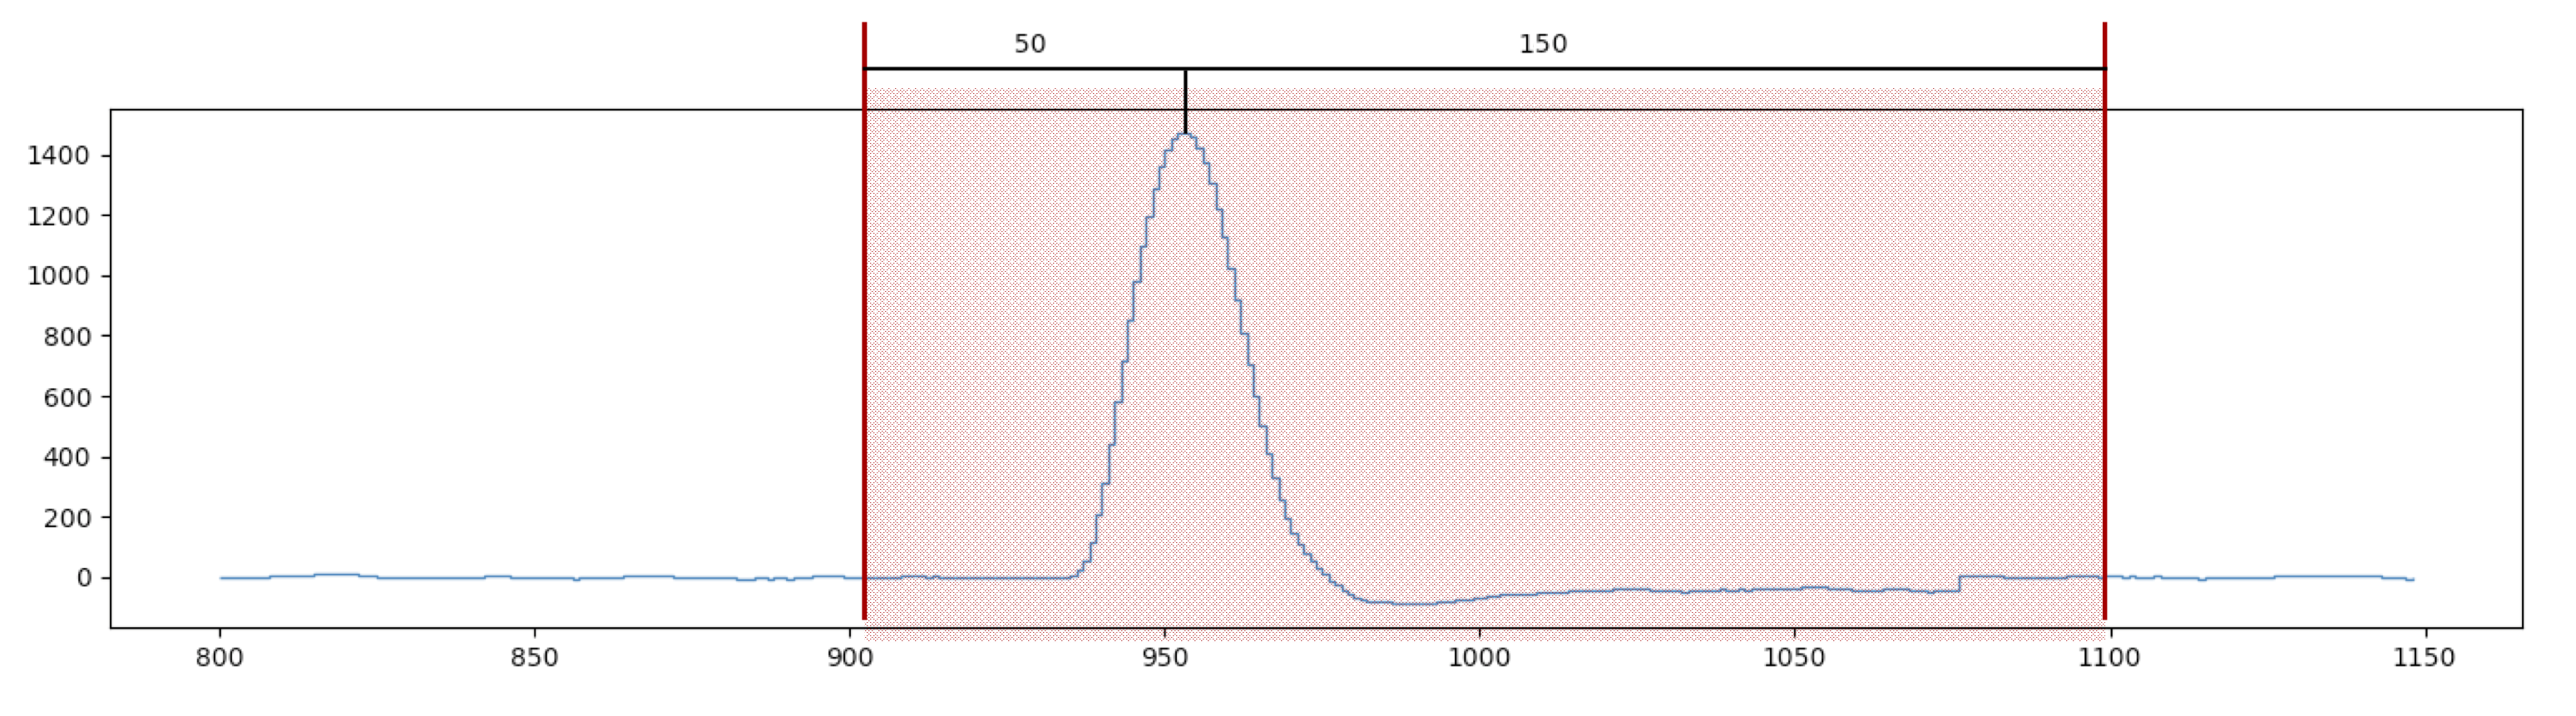
\includegraphics[width=\textwidth]{Pedestal}
  \caption{Схема расчета значений пьедесталов.}
  \label{fig:galaxy}
\end{figure}

    \subsection{Графический интерфейс}
    Здесь будет про графический интерфейс

    \subsection{Калибровка онлайн монитора светимости}
      Формы сигналов, которые получает монитор светимости имеют размерность в единицах АЦП на канал. Необходимо получать значения в энергетических единицах. Следовательно, стоит задача определения цены деления АЦП для каждого канала. Для этой цели была разработана процедура энергетической калибровки онлайн монитора светимости. Процедура основывается на посылке тестового сигнала и сравнения амплитуд с монитора светимости и уже откалиброванной системой DAQ. Калибровочные коэффициенты рассчитываются следующим образом:
\begin{equation}
  \eta = \frac{A_{DAQ}}{A_{LOM}}
\end{equation}
 где $A_{DAQ}$ и $A_{LOM}$ амплитуды с системы сбора данных DAQ и монитора светимости соответственно.\par
  Подробная схема данной процедуры представлена на рисунке 11 и заключается в следующем:
\begin{enumerate}
  \item На электромагнитный калориметр при помощи генератора импульсов подается тестовый сигнал
  \item Далее сигнал проходит все системы до монитора светимости как реальный сигнал
  \item На выходе с монитора светимости получаем амплитудные значения в каналах АЦП
  \item Далее вычисляются калибровочные коэффициенты по формуле (2)
\end{enumerate}\par
\begin{figure}[htp]
  \centering
  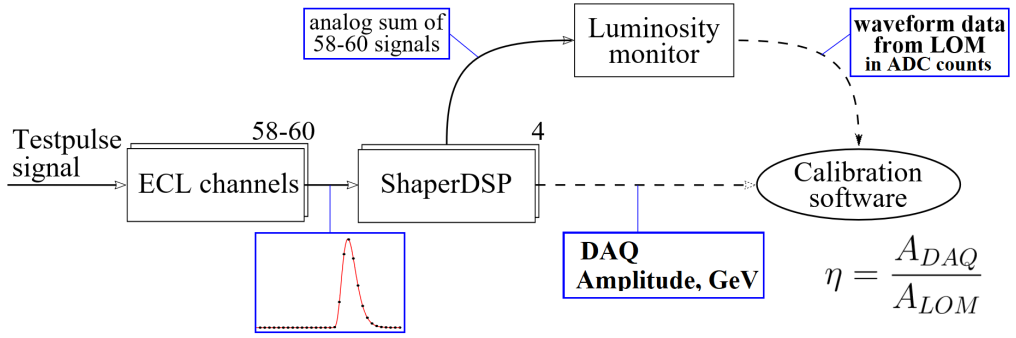
\includegraphics[width=\textwidth]{calibration.png}
  \caption{Процесс энергетической калибровки монитора светимости.}
  \label{fig:galaxy}
\end{figure}
  Так как в процессе энергетической калибровки необходимо параллельно читать данные с монитора светимости и амплитудные значения с системы сбора данных DAQ, то нужно иметь возможность управлять чтением данных с монитора светимости. Требуется останавливать и продолжать чтение данных в любой момент времени. Для реализации данной возможности был расширен протокол монитора светимости. Были добавлены команды, которые позволяют остановить чтение данных с монитора светимости, возобновить чтение данных и посмотреть текущий статус монитора светимости.\par
  Также для автоматизации контроля актуальной версии калибровочных коэффициентов, было реализовано хранение калибровочных коэффициентов в базе данных DAQ. При запуске ПО находит последнюю версию калибровочных коэффициентов и использует их в дальнейшем.\par
  В торцах электромагнитного калориметра находится 2112 кристаллов, однако, монитор светимости в конечном итоге получает суммированную информацию с этих каналов, сгруппированную по 32 секторам. Таким образом форма сигнала для каждого сектора -- это сумма форм сигналов от, в среднем, 2112/32 = 66 каналов. Однако, все кристаллы обладают немного разными физическими характеристиками, в частности, разным световыходом, требуется суммировать сигналы с неким весом. Этот вес называется коэффициентом аттенюации. Проанализировав изменения аттенюаторных и калибровочных коэффициентов, было замечено, что они коррелируют друг с другом. Поэтому, для более детального анализа, было проведен анализ изменения аттенюаторных коэффициентов и калибровочных за одинаковые промежутки времени. Результат сравнения представлен на рисунке 12. Таким образом, можно проверять, если изменились аттенюаторные коэффициенты, то на соответствующую величину изменять и калибровочные коэффициенты. Видно, что для некоторых секторов, к примеру секторов 1 и 28, корреляция не наблюдается, поэтому процедура автоподстройки коэффициентов является только вспомогательной операцией по отношению к калибровке. Тем не менее, эта процедура позволяет точнее исследовать вклад различных факторов, влияющих на цену деления АЦП.\par
  Также в случае возникновения проблем с соединением или считыванием значений из базы данных в компьютере, на котором запущено ПО, имеется офлайн версия калибровочных коэффициентов. Такой подход позволяет функционировать ПО независимо от соединения с БД.
\begin{figure}[htp]
  \centering
  \includegraphics[width=\textwidth]{coefs_new.pdf}
  \caption{Изменение калибровочных и аттенюаторных коэффициентов за равный промежуток времени.}
  \label{fig:galaxy}
\end{figure}


\section*{Заключение}
А здесь заключение

\section*{Список литературы}

\end{document}
